% Chapter 3 -- Data Acquisition and Dataset Construction
% Figures are authored in TikZ so the chapter compiles without external assets.
% Placeholders [VERIFY: ...] and [CITATION: ...] mark items still to be resolved.

\label{ch:data}

\tikzset{
  blk/.style={draw, rounded corners=2pt, align=center, inner sep=4pt,
              minimum height=8mm, font=\footnotesize},
  grp/.style={draw, dashed, rounded corners=3pt, inner sep=6pt},
  flow/.style={-{Latex[length=2mm]}, thick},
}

This chapter explains the process used to create the multimodal dataset used in
the remainder of this thesis. It introduces the wearable sensing platform and its
resource envelope, the assembly scenario, the activity classes recorded, the
firmware that streamed inertial and acoustic data off the devices, the protocol
used to record participants, the video-based annotation procedure, and the steps
of signal conditioning and windowing that transform the raw streams into labelled
two-second segments. The chapter ends with a quantitative characterisation of the
resulting dataset and an assessment of its known limitations. The modelling
choices made on this dataset are deferred to Chapter~\ref{ch:method}, and the
implications of the dataset's limitations for the validity of the results are
addressed in Chapter~\ref{ch:discussion}.

\section{Sensor Platform and Computational Constraints}
\label{sec:platform}

The sensing platform is the M5StickC Plus2, a self-contained wearable device built
around the ESP32-PICO-V3-02 system-on-chip (SoC), a dual-core processor clocked
up to 240\,MHz~\cite{m5stickcplus2}. Each device is equipped with a six-axis
inertial measurement unit (IMU, MPU6886) providing three-axis acceleration and
three-axis angular velocity, a digital MEMS microphone (SPM1423), a small
display, a single-cell 200\,mAh lithium-polymer battery, and a 2.4\,GHz Wi-Fi
radio~\cite{m5stickcplus2}.

\begin{figure}[!ht]
\centering
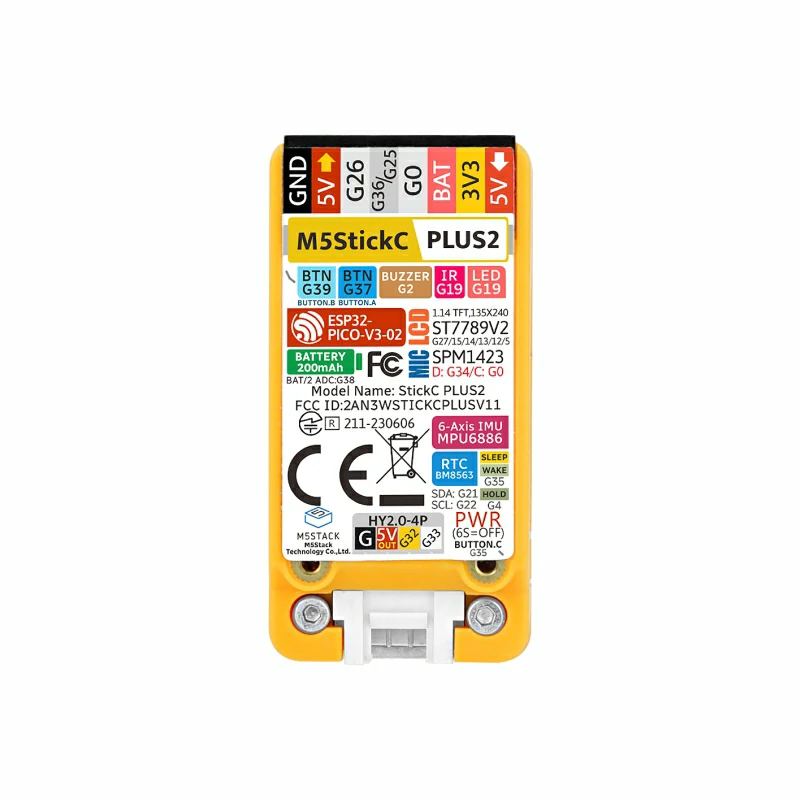
\includegraphics[width=0.4\textwidth]{figures/fig-m5stickc-plus2}
\caption{The M5StickC Plus2 wearable device. The ESP32-PICO-V3-02 system-on-chip,
the six-axis IMU (MPU6886), and the microphone (SPM1423) are all integrated on the
board. Image: M5Stack~\cite{m5stickcplus2}.}
\label{fig:m5stickc-plus2}
\end{figure}

Two properties of this platform shape the entire data pipeline. The first is that
the device is worn on the body, which rules out a high-bandwidth tethered
connection and makes wireless streaming the practical way to obtain data from
several body locations simultaneously. The second is the limited on-chip memory:
the manufacturer datasheet gives 8\,MB of flash, 2\,MB of in-package PSRAM, and
520\,KB of on-chip SRAM. This budget is comfortable for buffering and forwarding sensor samples during
acquisition, but it is the binding constraint on the eventual on-device inference
stage treated in Section~\ref{sec:deployment}. The dataset was therefore
designed so that the same device that records the training data can, in
principle, run the trained model: the inertial and acoustic sampling rates, the
window length, and the feature representations described later in this chapter
were all chosen with that target in mind rather than for offline convenience.

During data collection both the microphone and the IMU were used. The microphone
is single-channel, so each device produced one monophonic audio stream alongside
its six-axis inertial stream.

\section{Assembly Scenario and Activity Taxonomy}
\label{sec:taxonomy}

Recordings were carried out in the Future Work Lab at Fraunhofer IPA in Stuttgart,
a laboratory configured for research on human--machine interaction in
manufacturing {[}CITATION{]}.
The environment provides a workbench with parts, hand tools, and fasteners, so
that a manual assembly task can be performed under controlled but realistic
conditions.

Data were recorded from two participants over three sessions. In each session one
participant wore the sensors and performed the task while the other operated a
handheld mobile-phone camera, following the acting participant on foot during the
segments that involved walking; the two participants exchanged roles for later
sessions. Each session consisted of a repeated assembly sequence: three
repetitions in two of the sessions and four repetitions, plus one sequence marked
invalid, in the third. Session lengths, measured from the recorded streams, were
approximately 6.7, 7.6, and 16.9 minutes, for a total of about 31 minutes of
recording (Section~\ref{sec:protocol}).

Each repetition followed the same 32-step protocol, transcribed in the annotation
records. The participant begins at the bench, walks to a supply table, and
carries parts back; stacks three parts so that they align; seats them with a
hammer; measures the assembly with a scale; passes four screws through the
aligned parts by hand; drives the screws with a powered screwdriver; and places
the finished item in a storage compartment beside the bench. The remainder of
each repetition reverses the process, loosening and removing the screws and
returning the parts to their boxes. Because the same operations recur several
times per repetition, the screwdriving class dominates the dataset
(Section~\ref{sec:stats}).

Video of each session was annotated with a larger set of labels than the dataset
finally uses. Across sessions the coded label set contained fifteen to eighteen
activity labels, including narration (\texttt{speech}), the disassembly actions
(\texttt{screw\_loosening}, \texttt{remove\_screws}, \texttt{store\_part}), a rare
\texttt{pick\_container} action, and in one session the postures \texttt{sit} and
\texttt{stand}. The modelling taxonomy retains the ten classes listed in
Table~\ref{tab:activity-classes}, which cover the assembly half of the task
together with locomotion and rest. \texttt{screw\_loosening} was merged into
\texttt{screw\_tightening}: the two actions use the same powered screwdriver and
differ only in rotation direction, producing near-identical inertial and acoustic
signatures that a two-second window cannot reliably separate. This merge accounts
for the class's size: the 518 \texttt{screw\_tightening} windows in
Table~\ref{tab:activity-classes} include both tightening and loosening instances.
The remaining labels (\texttt{speech}, \texttt{remove\_screws},
\texttt{store\_part}, \texttt{pick\_container}, and, in one session,
\texttt{sit}/\texttt{stand}) were excluded rather than merged. The class
descriptions in Table~\ref{tab:activity-classes} are operational summaries taken
from the 32-step protocol; the typical instance duration is the mean length of a
coded activity segment, averaged over the three sessions.

\begin{table}[htbp]
\centering
\small
\setlength{\tabcolsep}{3.5pt}
\renewcommand{\arraystretch}{1.15}
\begin{tabularx}{\textwidth}{|p{2.4cm}|X|c|r|}
\hline
\textbf{Class} & \textbf{Operational description (from the recording protocol)}
 & \textbf{Typ.\ dur.} & \textbf{Win.} \\
\hline
\texttt{idle} & Standing at the bench without performing a task. & 4--12\,s & 45 \\
\texttt{walk} & Walking between the workstation and the supply table. & $\approx$5\,s & 73 \\
\texttt{carry\_\allowbreak container} & Carrying the parts container between the supply table and the workstation. & 5--9\,s & 56 \\
\texttt{place\_\allowbreak container} & Setting the parts container down on the work surface. & 3--5\,s & 35 \\
\texttt{assemble\_\allowbreak parts} & Stacking three parts on the workstation so that they align and fit together. & 10--19\,s & 143 \\
\texttt{hammering} & Striking the stacked parts with a hammer to seat them. & 6--11\,s & 85 \\
\texttt{measuring} & Measuring the length and width of the assembled part with a scale. & 8--9\,s & 93 \\
\texttt{insert\_\allowbreak screws} & Passing four screws through the aligned parts by hand. & 19--22\,s & 219 \\
\texttt{screw\_\allowbreak tightening} & Driving screws with a powered screwdriver; includes loosening actions merged into this class (Section~\ref{sec:taxonomy}). & 22--31\,s & 518 \\
\texttt{compartment\_\allowbreak interaction} & Opening and closing the storage compartment beside the bench. & 5--11\,s & 113 \\
\hline
\multicolumn{3}{|l|}{\textbf{Total paired windows}} & \textbf{1380} \\
\hline
\end{tabularx}
\caption{Activity classes in the modelling dataset. Descriptions are taken from
the 32-step assembly protocol. ``Typ.\ dur.'' is the range of mean coded-segment
durations across the three recording sessions; for \texttt{screw\_tightening} it
covers both the tightening and the merged loosening segments. ``Win.'' is the
number of two-second windows per class in the final dominant-wrist dataset
(Section~\ref{sec:stats}).}
\label{tab:activity-classes}
\end{table}

\section{Data-Collection Firmware}
\label{sec:firmware}

The same custom firmware was installed on all of the devices, written in C++ and
based on the Arduino framework. Its only task during acquisition is to sample the
two sensors and forward every sample to a host computer with enough timing
information for the streams to be reassembled and aligned afterwards. It performs
no filtering, no feature extraction, and no on-device storage. This section
explains the data acquisition architecture and the decisions behind it, rather
than the source code.

\subsection{Dual-Stream UDP Architecture}
\label{sec:udp}

The inertial and acoustic data are transmitted as two separate streams over
Wi-Fi using the User Datagram Protocol (UDP). One port receives inertial packets
and another receives audio packets, so that a receiver does not need to inspect
packet contents to separate the two modalities. UDP was preferred to a
connection-oriented protocol since it introduces no retransmission or reordering
delay, keeping the sender simple and the timing of transmitted packets close to
the timing of the underlying samples; the trade-off is that lost packets are not
retransmitted by the transport and must be detected and handled in post-processing
{[}CITATION{]}.

Each time a new IMU sample becomes available, an inertial packet is created that
contains the six inertial values as text, a sequence number, and a device
timestamp. Each audio packet has a sequence number, a sample count, a device
timestamp, and a fixed-size block of pulse-code-modulated (PCM) samples. Since
multiple devices send to the same host on the same two ports, the receiver logs
the source address of each packet it receives and uses it to differentiate the
streams by device. Figure~\ref{fig:acq-architecture} shows the end-to-end
acquisition path.

\begin{figure}[!ht]
\centering
\makebox[\textwidth][c]{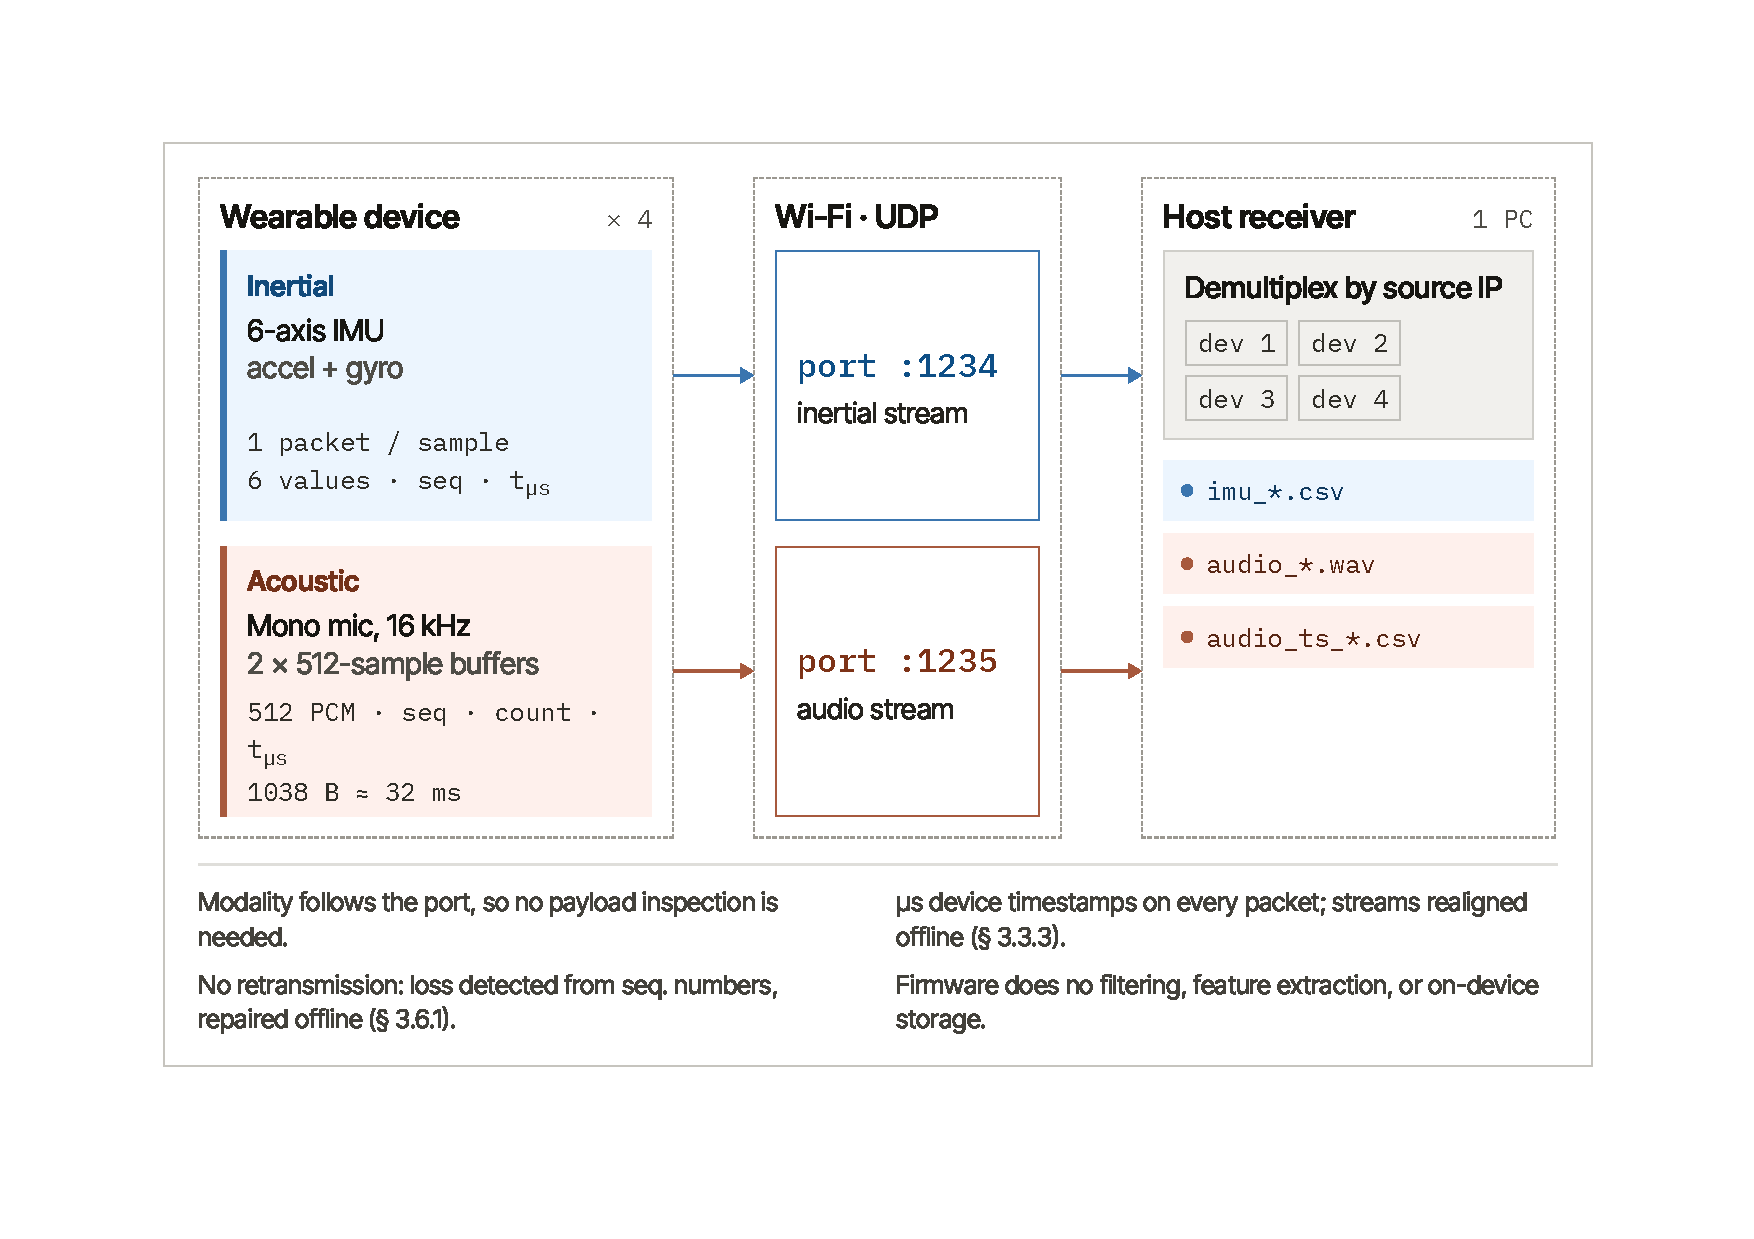
\includegraphics[width=1.1\textwidth]{figures/fig-acq-architecture}}
\caption{Architecture of the multimodal data-acquisition system. Each of the four
wearable devices samples an IMU and a microphone independently, timestamps and
frames the samples, and streams them as two separate UDP streams (inertial on one
port, audio on another) to a single host, which separates the devices by packet
source address and writes raw per-device files.}
\label{fig:acq-architecture}
\end{figure}

\subsection{Audio Double-Buffering and Packet Framing}
\label{sec:buffering}

Audio is captured continuously, so the firmware cannot stall the microphone
driver while a packet is being transmitted. To avoid this, two 512-sample buffers
are used alternately: while the driver fills one buffer, the previously filled
buffer is transmitted, and once a buffer is full, the roles swap. This prevents
new samples from overwriting data that has not yet been transmitted and keeps the
capture cadence regular.

The buffer size also determines the size of each audio packet. A 512-sample
block at a 16\,kHz sampling rate corresponds to 32\,ms of audio. Together with a
header carrying the sequence number, sample count, and timestamp, this produces a
packet of 1038\,bytes, which is well below the 1500-byte Ethernet MTU (Maximum
Transmission Unit), so every audio packet can be transmitted as a single,
unfragmented UDP datagram. Keeping packets under the MTU matters because IP
fragmentation of a UDP datagram means that losing any one fragment discards the
whole datagram, which can increase the effective audio packet loss rate
{[}CITATION{]}.

\subsection{Microsecond Timestamping and Sequence Numbering}
\label{sec:timestamps}

Each packet, inertial and acoustic, carries a timestamp taken from the device's
microsecond counter at the moment the packet is assembled, together with a
monotonically increasing sequence number. These two fields serve different
purposes. The sequence number makes packet loss detectable: a gap between
consecutive received sequence numbers means a lost packet, independent of any
timing assumption. The timestamp makes the true timing of a recording session
recoverable: it allows the elapsed time between the first and last samples to be
determined, which is later used for clock-drift correction in
Section~\ref{sec:conditioning}. It also provides the temporal reference needed to
align the inertial and acoustic streams from the same device.

The microsecond resolution is more than sufficient for this purpose: it is far
finer than the interval between individual inertial samples and than the interval
between consecutive audio packets, so timestamp quantisation does not introduce a
meaningful limitation to the alignment accuracy. The devices' timestamps cannot be
compared directly with one another, however, since the individual devices do not
share a common clock. The video reference described in
Section~\ref{sec:annotation} is therefore used to synchronise the various
devices.

\subsection{Multi-Device Capture and Body Placements}
\label{sec:placements}

In each recording session, four sensor devices were worn: one on the dominant
wrist, one on the non-dominant wrist, one at the waist, and one on the leg. All
four devices simultaneously recorded inertial and acoustic data and streamed
them to the host system. Recording at several body locations was a deliberate
design choice: it made it possible to capture potentially useful information
from different parts of the body and offered redundancy against a device failing
during a recording session.

However, not all of the recorded data were used to train the model.
Table~\ref{tab:placements} summarises the sensor data recorded and the data
finally input to the modelling pipeline. The models presented in this thesis use
only the dominant-wrist inertial data and the dominant-wrist microphone data.

During preprocessing, windows were first created for all four sensor locations
and placed in their respective session directories. These windows used the same
naming convention across all placements, based on the activity, window start
time, and window index on the shared video-aligned timeline. This naming
convention persisted when the windows were subsequently consolidated into one
directory, so each window was retained as a single file. A byte-level comparison
of the retained inertial and audio files indicated that they are those of the
dominant-wrist device. Non-dominant-wrist, waist, and leg data are thus available
in the original session data, but not in the modelling dataset.

The data from the leg-worn sensor package were excluded after inspection of the
recorded signals. The leg inertial data contained relatively little
activity-specific information for the bench-based assembly tasks, apart from
activities such as walking. Likewise, the leg microphone primarily recorded
ambient noise and captured the assembly activities poorly. This thesis also did
not use the inertial data of the non-dominant wrist and waist as model inputs.
Integrating information across more than one body location, at the feature level
or at the decision level, is instead noted as a direction for future work,
addressed in Chapter~\ref{ch:conclusion}.

\begin{table}[htbp]
\centering
\renewcommand{\arraystretch}{1.2}
\begin{tabularx}{\textwidth}{|l|C|C|C|}
\hline
\textbf{Placement} & \textbf{Modalities recorded}
 & \textbf{IMU as model input} & \textbf{Audio as model input} \\
\hline
Dominant wrist     & inertial + audio & yes & yes \\
Non-dominant wrist & inertial + audio & no  & no  \\
Waist              & inertial + audio & no  & no  \\
Leg                & inertial + audio & no  & no  \\
\hline
\end{tabularx}
\caption{Body placements: data recorded during acquisition versus data used as
model input in the final pipeline. Only the dominant-wrist inertial and acoustic
streams reach the model.}
\label{tab:placements}
\end{table}

\section{Recording Protocol}
\label{sec:protocol}

The same procedure was followed for each recording session. All four devices
were worn by the acting participant and fastened with straps to keep the sensor
axes fixed relative to the body segment to which they belonged. Before recording
started, all devices were checked to ensure that they were connected and
transmitting data correctly. The participant then repeated the set of predefined
assembly steps at the workbench while the second participant filmed the assembly
sequence with a handheld phone. The host computer displayed the incoming packets
from all four devices, so that a disconnection or a sustained loss of packets
could be noticed; no session required a restart.

Table~\ref{tab:sessions} provides an overview of the recorded sessions. The
session durations were calculated from the recorded inertial streams, and the
number of two-second windows was counted from the final dataset. The three
sessions contributed 352, 371, and 657 windows. This class imbalance, as
discussed in Section~\ref{sec:stats}, is mostly due to the recording protocol:
some actions, such as screwdriving, were performed several times within each
repetition, whereas other actions, such as placing a container, occurred only
once per repetition.

\begin{table}[htbp]
\centering
\small
\setlength{\tabcolsep}{4pt}
\renewcommand{\arraystretch}{1.2}
\begin{tabular}{|c|p{3.9cm}|c|c|c|}
\hline
\textbf{Part.} & \textbf{Session (project label)} & \textbf{Duration}
 & \textbf{Reps} & \textbf{Windows} \\
\hline
P2 & First session, all four placements & $\approx$6.7\,min & 3 & 352 \\
P1 & Three repetitions                  & $\approx$7.6\,min & 3 & 371 \\
P2 & Four repetitions, one invalid      & $\approx$16.9\,min & 4\,$(+1)$ & 657 \\
\hline
\multicolumn{2}{|l|}{\textbf{Total}} & \textbf{$\approx$31.2\,min} & & \textbf{1380} \\
\hline
\end{tabular}
\caption{Data-acquisition sessions. ``Session'' paraphrases the folder label used
in the project records. ``$(+1)$'' denotes one further sequence marked invalid and
set aside.}
\label{tab:sessions}
\end{table}

\section{Ground-Truth Annotation from Synchronised Video}
\label{sec:annotation}

The sensor recordings provide motion and acoustic information but do not contain
activity labels. The ground truth was therefore obtained from the recorded
video, which provides a visual reference for determining which activity was
being performed at a given point in time. The annotated video intervals were
then transferred to the sensor recordings. This process requires the video and
sensor data to be placed on a common timeline and the activities to be
represented as defined time intervals.

\subsection{Determination of the Audio-Video Offset}
\label{sec:offset}

The video and sensor recordings were started independently, meaning that their
time origins were not identical. Before the video annotations could be mapped
to the sensor data, a temporal offset between the two recordings had to be
determined.

The offset was calculated by finding an event that is clearly identifiable in
both the video and the recorded audio. The audio from the sensor side was
analysed in Audacity~\cite{audacity} to find the corresponding transient, which
was located within a millisecond. The same event, a spoken cue that the
participant announced at the start and end of each assembly sequence, was then
found in the video's audio track. The difference between the event times in the
sensor recording and the video provides the required temporal offset.

For instance, the offset measured for one session is 3.857\,seconds. This value
is used for the synchronisation procedure to take out the same amount of data
from the beginning of each sensor stream, so that the beginning of the sensor
timeline becomes the zero point of the video. In each recording session, the
offset was determined independently and applied to the synchronised streams used
in this thesis. This step appears in the full preprocessing pipeline shown in
Figure~\ref{fig:pipeline}.

\subsection{Interval Labels and Sample-Level Label Embedding}
\label{sec:labels}

The activities were annotated directly from the video using
BORIS~\cite{friard2016boris}, a tool for behavioural observation and event
logging. Every annotation specifies a start time, an end time, and an activity
label on the video timeline. The annotations were exported to a table with the
columns \texttt{Label}, \texttt{Start}, and \texttt{End}.

These annotation intervals were then moved to the sensor data. For each
inertial sample, its timestamp relative to the beginning of the recording was
compared with the annotated intervals. If the timestamp was within an activity
interval, the associated activity label was attributed to the sample. Samples
that were not part of any of the annotated intervals were assigned a reserved
\texttt{unlabeled} marker. This avoids assigning an activity label to
transition periods or moments in which no specific task was being performed.

The assigned label was saved as a separate column along with the inertial
measurements, and thus the inertial recording was transformed into a labelled
time series. The audio stream was labelled using the same temporal reference.
Since the audio and inertial data originate from the same device and were
aligned to the video timeline, an audio segment corresponds to the activity
represented by the inertial samples covering the same time interval.
Consequently, transitions and untasked periods remain explicitly represented as
\texttt{unlabeled}. Their treatment during the subsequent windowing process is
described in Section~\ref{sec:windowing}.

\section{Signal Conditioning}
\label{sec:conditioning}

Before the data were divided into windows, the recorded streams were processed
to compensate for transmission-related artefacts and differences in the device
clocks. Next, the inertial and acoustic data were brought to fixed sampling
rates to ensure consistent processing across all the recordings.

The conditioning process was repeated for each of the devices and yielded
continuous, uniformly sampled, and temporally aligned inertial and acoustic
streams. The entire pre-processing chain is shown in Figure~\ref{fig:pipeline}.

\begin{figure}[htbp]
\centering
\begin{tikzpicture}[node distance=3.5mm, every node/.style={blk, text width=6.6cm}]
  \node (raw) {Per-device raw streams (\texttt{imu}, \texttt{audio}, \texttt{audio\_ts})};
  \node (drop) [below=of raw] {Audio-dropout detection; silent (zero) padding of missing chunks};
  \node (drift) [below=of drop] {Clock-drift correction: sample rate re-estimated from first/last timestamp};
  \node (trim) [below=of drift] {Inertial head-trim to the audio start time};
  \node (vid) [below=of trim] {Video-offset trim to the annotation zero mark};
  \node (lab) [below=of vid] {Interval-label embedding (BORIS export)};
  \node (split) [below=of lab, text width=6.6cm]
        {Inertial: mean-bin decimation to 80\,Hz \quad$|$\quad Audio: resample to 16\,kHz};
  \node (seg) [below=of split] {Continuous activity-segment extraction ($\geq 2$\,s)};
  \node (win) [below=of seg] {Two-second windowing, 50\,\% overlap, majority-vote label, $\geq 70$\,\% label coverage};
  \node (out) [below=of win] {Labelled paired inertial/audio windows};
  \foreach \a/\b in {raw/drop, drop/drift, drift/trim, trim/vid, vid/lab, lab/split,
                     split/seg, seg/win, win/out}
    \draw[flow] (\a) -- (\b);
\end{tikzpicture}
\caption{Signal-conditioning and windowing pipeline, applied per device. The
inertial and acoustic branches are brought to fixed rates before both are cut on
the same window boundaries.}
\label{fig:pipeline}
\end{figure}

\subsection{Packet-Loss Detection and Audio-Dropout Reconstruction}
\label{sec:dropout}

Missing audio packets appear as gaps in the recorded waveform. Since each audio
packet contains an arrival timestamp and a fixed number of samples, the
expected time between consecutive packets can be determined. At a sampling rate
of 16\,kHz, for example, a packet containing 512 samples represents 32\,ms of
audio, so under normal conditions consecutive packets are expected to be
separated by approximately 32\,ms.

A larger time gap between two received packets indicates that one or more
packets may have been lost. The number of missing packets is estimated from the
observed time difference using
\[
\operatorname{round}\!\left(\frac{\Delta t - T_{\mathrm{packet}}}{T_{\mathrm{packet}}}\right),
\]
where $\Delta t$ denotes the observed time difference between two consecutive
received packets and $T_{\mathrm{packet}}$ denotes the expected packet
interval. For the 16\,kHz audio stream with 512 samples per packet,
$T_{\mathrm{packet}} = 32\,\mathrm{ms}$. For example, if two received packets
are separated by 96\,ms, the equation gives
\[
\operatorname{round}\!\left(\frac{96 - 32}{32}\right) = 2.
\]
This means that two packets are assumed to be missing between the two received
packets.

If a packet is detected as missing, a block of 512 zero-valued samples is
inserted at the appropriate location in the waveform. This approach does not
attempt to reconstruct the missing acoustic content. Instead, its purpose is to
preserve the correct duration and temporal position of the surrounding signal
so that subsequent time-frequency analysis is not affected by a shortened audio
stream. The missing regions are therefore represented as silence. This is a
conservative approach, as it introduces no artificial acoustic events, at the
cost of a short period of artificially silent audio.

The fraction of reconstructed audio, computed from the raw per-device
packet-arrival timestamps, is 0.15--0.40\,\% per session and about 0.33\,\%
overall for the dominant wrist (Section~\ref{sec:quality}); this is numerically
identical to the packet-loss rate, since every missing packet is exactly 512
samples of silence.

The sequence numbers are used to detect the loss of packets in the inertial
streams as well. In the dominant-wrist stream, the packet-loss rates were
0.056\,\%, 0.022\,\%, and 0.031\,\% for the three sessions, respectively, and
roughly 0.035\,\% overall (Section~\ref{sec:quality}). As described in
Section~\ref{sec:decimation}, the short gaps in the inertial data were then
filled by linear interpolation on the resampled time grid.

\subsection{IMU Decimation to 80\,Hz}
\label{sec:decimation}

The inertial stream is delivered at the device native rate, measured at
249.6--249.9\,Hz across the three sessions from the devices' microsecond
timestamps. This is consistent with the recovered design notes but not with the
firmware's own in-code comment, which labels the relevant configuration call
``100\,Hz''; the discrepancy has no effect on the modelling data, since
decimation always targets a fixed 80\,Hz regardless of the input rate. The
stream is reduced to this uniform 80\,Hz for modelling.

The reduction is performed by mean binning. The stream is divided into
consecutive 12.5\,ms bins, matching the desired sampling period at 80\,Hz, and
the inertial values in each bin are averaged to produce one output sample. If a
bin contains no samples, for instance because of packet loss, its value is
estimated by linear interpolation between the surrounding samples. The label
column is decimated separately by taking the most frequent label in each bin.
The resulting stream sits on an exact 80\,Hz grid, which removes the small
timing irregularities of the native stream.

Mean binning also provides a simple form of smoothing, although it is not used
as a substitute for a specifically designed anti-aliasing filter. In
particular, averaging within each bin attenuates signal components above the
new Nyquist frequency of 40\,Hz to some degree, but no filter with a defined
passband or stopband was designed as part of this preprocessing step.

The rate of 80\,Hz was selected based on the target platform and the
anticipated nature of the activities to be captured. The sampling rate is
intended to retain the frequency content relevant to the wrist movements
involved in manual assembly, while substantially reducing the amount of
inertial data and the resulting model input size {[}CITATION{]}. This
reduces the inertial sampling rate by roughly a factor of three compared with
the measured native rate.

\subsection{Audio Resampling to a Strict 16\,kHz Timeline}
\label{sec:resample}

Following clock-drift correction, every audio stream is resampled from its
effective sampling rate to a strict 16\,kHz timeline using the band-limited
resampler in librosa~\cite{mcfee2015librosa}. The resulting signal is stored as
16-bit PCM.

Using a fixed sampling rate ensures that the number of audio samples directly
corresponds to a fixed duration. This is crucial for the windowing and
feature-extraction stages that follow, because each example must span the same
time interval and generate a consistent input representation. The sampling
rate of 16\,kHz is also sufficient to capture the frequency range considered
relevant for the recorded assembly activities, which include impulsive and
periodic sounds such as those generated when hammering and screwdriving. It is
also consistent with the sampling rate used by the audio feature-extraction
pipeline described in Chapter~\ref{ch:method}.

\section{Window Generation and Labelling}
\label{sec:windowing}

After signal conditioning, the synchronised streams are first cut into
continuous activity segments. Each segment is associated with one annotated
activity interval and is only considered for further processing if it has a
duration of at least two seconds. These segments are later split into
equal-size windows for classification.

Each window has a duration of two seconds, with a 50\,\% overlap between
consecutive windows, so a new window starts every one second. Overlapping
windows are common in activity recognition because they increase the number of
training examples and reduce the chance that a short activity is sliced at a
window boundary~\cite{bulling2014tutorial}; the selected two-second window
length and 50\,\% overlap are within the range commonly used in wearable
HAR~\cite{banos2014window}. For the selected sampling rates, each two-second
window contains 160 inertial samples at 80\,Hz and 32\,000 audio samples at
16\,kHz. Both modalities are segmented using the same temporal boundaries on
the shared timeline, so each inertial window has a corresponding audio window
of the same span; the two together form one paired multimodal example.

The activity label of each window is decided using majority vote. The vote
counts only samples that carry a valid activity label; samples tagged as
\texttt{unlabeled} (Section~\ref{sec:labels}) are not included. The activity
that appears most often among the labelled samples is assigned to the window.

To prevent transition periods from becoming part of the training data, a
minimum label-coverage threshold of 70\,\% is applied. A window is kept only if
at least 70\,\% of its samples have a valid activity label. A window with a high
proportion of \texttt{unlabeled} samples is not assigned to an activity class
but is discarded instead, usually at transitions between activities. This
method keeps windows with many transitions out of the training data while
preserving windows that may have some activity-boundary overlap.
Figure~\ref{fig:windowing} shows the full window generation and labelling
process.

\begin{figure}[htbp]
\centering
\resizebox{\textwidth}{!}{%
\begin{tikzpicture}[x=1cm, y=1cm, font=\scriptsize]
  % labelled stream strip: 1 cm == 1 s
  \fill[black!8]  (0,0)   rectangle (3,0.6);
  \fill[black!22] (3,0)   rectangle (6.5,0.6);
  \fill[pattern=north east lines] (6.5,0) rectangle (7.3,0.6); % unlabeled
  \fill[black!35] (7.3,0) rectangle (11,0.6);
  \draw (0,0) rectangle (11,0.6);
  \node at (1.5,0.3)  {activity A};
  \node at (4.75,0.3) {activity B};
  \node at (9.15,0.3) {activity C};
  \node[above] at (6.9,0.62) {unlabeled};
  \node[left] at (0,0.3) {stream};
  \draw[-{Latex[length=1.6mm]}] (0,-0.35) -- (11,-0.35) node[right] {time};
  % stacked 2 s windows (2 cm wide), each with its label to the right
  \foreach \y/\xa/\txt in {%
      -0.9/0.5/{$W_1$: 100\,\% A $\Rightarrow$ A},
      -1.5/2.0/{$W_2$: $\sim$75\,\% A, $\sim$25\,\% B $\Rightarrow$ A},
      -2.1/5.8/{$W_3$: $<$70\,\% labelled $\Rightarrow$ discarded}}{
    \pgfmathsetmacro{\xb}{\xa+2}
    \draw[|-|, thick] (\xa,\y) -- (\xb,\y);
    \node[right] at (\xb,\y) {\ \txt};
  }
\end{tikzpicture}}
\caption{Window generation and majority-vote labelling. Two-second windows advance
in one-second steps ($W_1$, $W_2$, $W_3$ shown stacked for clarity). A window takes
the majority activity among its labelled samples; a window whose labelled coverage
falls below 70\,\%, such as one spanning the transition region, is discarded.}
\label{fig:windowing}
\end{figure}

Windowing was carried out for all four body placements, producing one set of
labelled inertial and audio windows per placement, organised by class. The
per-placement sets that are not used for modelling contain fifteen activity labels
each.

\section{Dataset Statistics, Class Distribution, and Imbalance}
\label{sec:stats}

The dataset used for modelling is the dominant-wrist subset. It has 1380 paired
inertial and audio windows for the ten activity classes outlined in
Table~\ref{tab:activity-classes}. The data come from two participants and
three recording sessions and represent roughly 23 minutes of windowed activity
out of the 31 minutes of recorded data; the remaining time is not part of the
modelling dataset because of excluded classes, the invalid sequence, and
windows removed around activity transitions.

Each inertial window contains a $160 \times 6$ array of accelerometer and
gyroscope measurements sampled at 80\,Hz. Each corresponding audio window
contains 32\,000 mono samples at 16\,kHz. Table~\ref{tab:composition}
summarises the composition of the dataset, and Figure~\ref{fig:classdist}
shows the distribution of windows across the activity classes.

\begin{table}[htbp]
\centering
\begin{tabular}{|l|l|}
\hline
\textbf{Property} & \textbf{Value} \\
\hline
Paired inertial/audio windows & 1380 \\
Activity classes              & 10 \\
Participants                  & 2 \\
Recording sessions            & 3 \\
Windowed activity             & $\approx$23\,min \\
Window length                 & 2\,s \\
Window stride                 & 1\,s (50\,\% overlap) \\
Minimum label coverage        & 70\,\% \\
Inertial window               & $160 \times 6$ at 80\,Hz \\
Audio window                  & 32\,000 samples, mono, 16\,kHz \\
Inertial channels             & acc\_x, acc\_y, acc\_z, gyro\_x, gyro\_y, gyro\_z \\
\hline
\end{tabular}
\caption{Composition of the dominant-wrist modelling dataset.}
\label{tab:composition}
\end{table}

\begin{figure}[htbp]
\centering
\resizebox{\textwidth}{!}{%
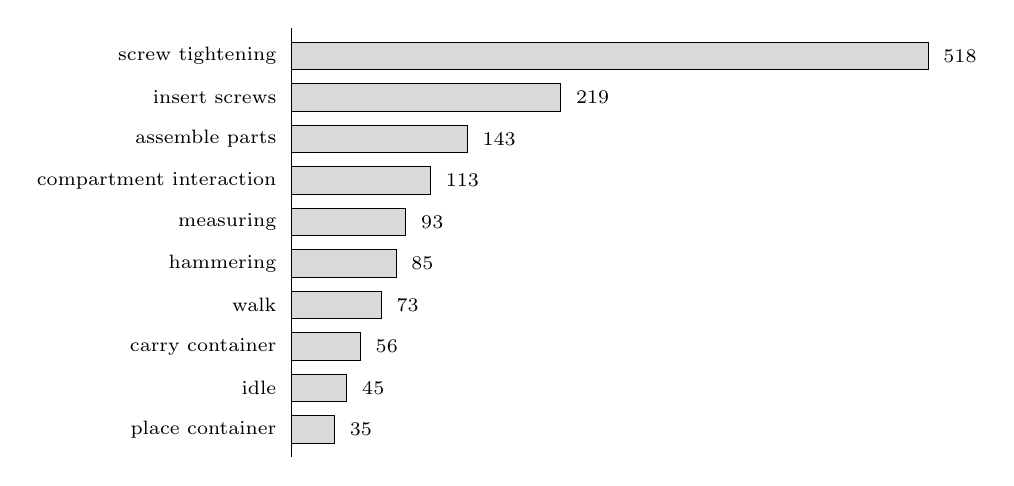
\begin{tikzpicture}[x=1pt, y=1pt]
  \foreach [count=\i] \name/\val in {%
      screw tightening/518, insert screws/219, assemble parts/143,
      compartment interaction/113, measuring/93, hammering/85, walk/73,
      carry container/56, idle/45, place container/35}{
    \pgfmathsetmacro{\w}{\val/518*230}
    \pgfmathsetmacro{\yb}{-\i*15}
    \pgfmathsetmacro{\yt}{\yb+10}
    \pgfmathsetmacro{\ym}{\yb+5}
    \pgfmathsetmacro{\wl}{\w+2}
    \fill[black!15] (0,\yb) rectangle (\w,\yt);
    \draw (0,\yb) rectangle (\w,\yt);
    \node[left,  font=\scriptsize] at (-2,\ym) {\name};
    \node[right, font=\scriptsize] at (\wl,\ym) {\val};
  }
  \draw (0,0) -- (0,-155);
\end{tikzpicture}}
\caption{Number of two-second windows per activity class in the dominant-wrist
dataset ($n = 1380$). The distribution is dominated by the screwdriving classes;
\texttt{screw\_tightening} alone accounts for about 38\,\% of the windows and the
two screwdriving classes together for more than half.}
\label{fig:classdist}
\end{figure}

There is a significant imbalance in the class distribution. The smallest
class, \texttt{place\_container}, contains only 35 windows, roughly one
fifteenth of the largest. This imbalance is primarily due to the design of the
task: actions such as screwdriving were repeated numerous times during each
session, while other activities such as moving a container or walking were
repeated only a few times. Consequently, the imbalance persists in the dataset
and is not corrected during preprocessing. How it is handled in training and
evaluation is detailed in Chapter~\ref{ch:method}, and its impact on the
findings in Chapter~\ref{ch:discussion}.

The number of windows discarded during windowing because they failed the
70\,\% label-coverage requirement was not recorded.

\section{Data-Quality Assessment and Known Artefacts}
\label{sec:quality}

There are a number of characteristics of the data that are important to
consider. These characteristics do not prevent the dataset from being used for
the experiments in this thesis, but they define the limits of what can
reasonably be concluded from those experiments. Table~\ref{tab:quality}
summarises the primary data-quality indicators that could be established.

\begin{table}[htbp]
\centering
\footnotesize
\setlength{\tabcolsep}{3.5pt}
\renewcommand{\arraystretch}{1.2}
\begin{tabularx}{\textwidth}{|p{3.5cm}|p{2.3cm}|X|}
\hline
\textbf{Indicator} & \textbf{Value} & \textbf{Notes} \\
\hline
Inertial packet loss (dominant wrist) & 0.022--0.056\,\% per session &
  From sequence-number gaps; $\approx$0.035\,\% overall. Below the 1\,\% design
  target. \\
Audio packet loss (dominant wrist) & 0.15--0.40\,\% per session; $\approx$0.33\,\% overall &
  From \texttt{audio\_ts} packet-arrival timestamp gaps, computed from the raw
  per-device logs. Reconstructed audio (inserted silence) is the same
  fraction, since every missing packet is exactly 512 samples. \\
Synchronisation basis & one manual event per session &
  Residual reading error and slow clock drift over a session are not
  characterised. \\
Camera & handheld, moving &
  Framing varied, but no hand action was occluded during annotation. \\
Discarded low-coverage windows & not recorded & See Section~\ref{sec:stats}. \\
\hline
\end{tabularx}
\caption{Data-quality indicators for the dataset.}
\label{tab:quality}
\end{table}

\textbf{Packet loss and audio reconstruction.} Wireless UDP transmission loses
packets. Inertial loss on the dominant-wrist stream is measured at about
0.035\,\% overall (Section~\ref{sec:dropout}). Audio loss, computed from the raw
per-device packet-arrival timestamps, is higher: 0.15--0.40\,\% per session and
about 0.33\,\% overall for the dominant wrist, roughly an order of magnitude
above the inertial loss rate. Because every missing audio packet is
reconstructed as exactly 512 samples of silence (Section~\ref{sec:dropout}), the
reconstructed-audio fraction is numerically the same figure.

\textbf{Synchronisation uncertainty.} The alignment of the sensor recordings
with the activity annotations is based on a manually identified synchronisation
event for each session, followed by a fixed offset applied to the entire
session (as described in Section~\ref{sec:offset}). There is no quantification
of the residual error caused by manual event locating, and no characterisation
of the gradual clock drift between the recordings. Majority voting applied over
two-second windows and the 70\,\% threshold for label coverage minimise the
risk of a small window alignment error affecting the label assigned to a
particular window. However, this kind of error can still change the effective
boundaries of an activity.

\textbf{Scope of the dataset.} The dataset was collected from two participants
performing a scripted assembly task in a single laboratory environment. The
final modelling data represent approximately 23 minutes of windowed activity,
with one class accounting for more than one third of all windows. The dataset
is suitable for the comparative analysis of multimodal fusion methods and
on-device feasibility undertaken in this thesis. Its size and limited variation
do not make it suitable for assessing how the resulting models would perform
for different participants, assembly tasks, or environments. These limitations
are addressed in more detail in Chapter~\ref{ch:discussion}, which also
discusses their effect on the experimental results.

\section{Chapter Summary}
\label{sec:ch3-summary}

This chapter described the construction of the multimodal dataset. Inertial and
acoustic data were streamed over Wi-Fi from four M5StickC Plus2 devices worn at the
wrists, waist, and leg, using a UDP-based firmware that timestamps and
sequence-numbers every packet so that the streams can be realigned after
transmission. Two participants performed a scripted manual assembly task across
three sessions in the Fraunhofer IPA Future Work Lab, alternating between
performing the task and filming it on a handheld phone. Activity intervals were
coded from the video in BORIS and transferred onto the sensor timeline after the
sensor-to-video offset was fixed from a shared event located in Audacity. Each
device stream was then corrected for audio dropouts and clock drift, decimated to
80\,Hz for the inertial channels and resampled to 16\,kHz for audio, and segmented
into overlapping two-second windows labelled by majority vote subject to a 70\,\%
coverage threshold. The modelling dataset used in the remainder of this thesis is
the dominant-wrist subset: 1380 paired inertial and audio windows over ten activity
classes, single-channel audio, with a strong class imbalance dominated by
screwdriving actions and with the data-quality limitations set out in
Section~\ref{sec:quality}. This dataset is the common input to all of the models
and experiments described in the following chapters.
